\documentclass[12pt]{article}

\usepackage{amsmath,amsthm,amsfonts,amssymb,amsxtra}
\usepackage{pgf,tikz}
\usetikzlibrary{arrows, calc}
\renewcommand{\theenumi}{(\alph{enumi})} 
\renewcommand{\labelenumi}{\theenumi}

\pagestyle{empty}
\setlength{\textwidth}{7in}
\setlength{\oddsidemargin}{-0.5in}
\setlength{\topmargin}{-1.0in}
\setlength{\textheight}{9.5in}

\theoremstyle{definition}
\newtheorem{problem}{Problem}

\begin{document}

\noindent{\large\bf MATH 241}\hfill{\large\bf Exam\#3.}\hfill{\large\bf
  Spring 2018}\hfill{\large\bf Page 1/6}\hrule

\bigskip
\begin{center}
  \begin{tabular}{|ll|}
    \hline & \cr
    {\bf Name: } & \makebox[12cm]{\hrulefill}\cr & \cr
    {\bf VIP ID:} & \makebox[12cm]{\hrulefill}\cr & \cr
    \hline
  \end{tabular}
\end{center}
\begin{itemize}
\item Write your name and VIP ID in the space provided above.
\item The test has six (6) pages, including this one.
\item The test is seventy-five (75) minutes long.
\item Enter your answer in the boxes provided.
\item You must show sufficient work to justify all answers unless
  otherwise stated in the problem.  Correct answers with inconsistent
  work may not be given credit.
\item Credit for each problem is given in parentheses at the right of
  the problem number.
\item No books, notes or calculators may be used on this test.
\end{itemize}
\hrule

\begin{center}
  \begin{tabular}{|c|c|c|}
    \hline
    &&\cr
    {\large\bf Page} & {\large\bf Max.~points} & {\large\bf Your points} \cr
    &&\cr
    \hline
    &&\cr
    {\Large 2} & \Large 20 & \cr
    &&\cr
    \hline
    &&\cr
    {\Large 3} & \Large 10 & \cr
    &&\cr
    \hline
    &&\cr
    {\Large 4} & \Large 10 & \cr
    &&\cr
    \hline
    &&\cr
    {\Large 5} & \Large 30 & \cr
    &&\cr
    \hline
    &&\cr
    {\Large 6} & \Large 30 & \cr
    &&\cr
    \hline\hline
    &&\cr
    {\large\bf Total} & \Large 100 & \cr
    &&\cr
    \hline
  \end{tabular}
\end{center}
\newpage

%%%%%%%%%%%%%%%%%%%%%%%%%%%%%%%%%%%%% Page 2
\noindent{\large\bf MATH 241}\hfill{\large\bf Exam\#3.}\hfill{\large\bf
  Spring 2018}\hfill{\large\bf Page 2/6}\hrule

\bigskip
\begin{problem}[10 pts]
Evaluate $\displaystyle{\int_R (3x+4y^2)\, dA}$, where $R$ is the region in the upper half-plane bounded by the circles
$x^2+y^2=1$ and $x^2+y^2=4$.  Sketch the region of integration.

\vspace{1cm}
\begin{tikzpicture}[scale=0.7]
  \draw [white] (-0.5,-0.5) rectangle (6.5,6.5);
  \draw [<->, ultra thick] (-0.5,3) -- (6.5,3);
  \draw [<->, ultra thick] (3,-0.5) -- (3,6.5);
  \draw[step=0.5,gray,ultra thin] (-0.25, -0.25) grid (6.25, 6.25);
  \end{tikzpicture}
\begin{flushright}

\vspace{3cm}
  \begin{tikzpicture}
    \draw (-2cm, 0.5cm) node {$\displaystyle{\int_R (3x+4y^2)\, dA =}$};
    \draw (0cm,-0.2cm) rectangle (5cm,1.2cm);
  \end{tikzpicture}
\end{flushright}
\end{problem}
\hrule
\begin{problem}[10 pts]
Sketch the domain of integration, and convert the following integrals to polar coordinates.  \textbf{Do not evaluate.}
\begin{equation*}
\int_0^1 \int_0^y x\, dx\, dy = \framebox{\textcolor{white}{$\Bigg($} \hspace{9cm}}
\end{equation*}

  \vspace{0.25cm}
  \begin{tikzpicture}[scale=0.7]
  \draw [white] (-0.5,-0.5) rectangle (6.5,6.5);
  \draw [<->, ultra thick] (-0.5,3) -- (6.5,3);
  \draw [<->, ultra thick] (3,-0.5) -- (3,6.5);
  \draw[step=0.5,gray,ultra thin] (-0.25, -0.25) grid (6.25, 6.25);
  \end{tikzpicture}
\end{problem}
\newpage

%%%%%%%%%%%%%%%%%%%%%%%%%%%%%%%%%%%%% Page 3
\noindent{\large\bf MATH 241}\hfill{\large\bf Exam\#3.}\hfill{\large\bf
  Spring 2018}\hfill{\large\bf Page 3/6}\hrule

\bigskip
\begin{problem}[10 pts]
Evaluate the integral $\int_R \sin(y^2)\, dA$ where $R$ is the triangle with vertices $(0,0)$, $(1,1)$ and $(0,1)$. Sketch the domain of integration. \newline \textbf{Hint: The order of integration really matters for this problem.}

\vspace{0.5cm}
\begin{tikzpicture}[scale=0.7]
  \draw [white] (-0.5,-0.5) rectangle (6.5,6.5);
  \draw [<->, ultra thick] (-0.5,0) -- (6.5,0);
  \draw [<->, ultra thick] (0,-0.5) -- (0,6.5);
  \draw[step=0.5,gray,ultra thin] (-0.25, -0.25) grid (6.25, 6.25);
  \end{tikzpicture}
\begin{flushright}

\vspace{14cm}
  \begin{tikzpicture}
    \draw (-1.75cm, 0.5cm) node {$\displaystyle{\int_R \sin(y^2)\, dA =}$};
    \draw (0cm,-0.2cm) rectangle (6cm,1.2cm);
  \end{tikzpicture}
\end{flushright}
\end{problem}
\newpage

%%%%%%%%%%%%%%%%%%%%%%%%%%%%%%%%%%%%% Page 4
\noindent{\large\bf MATH 241}\hfill{\large\bf Exam\#3.}\hfill{\large\bf
  Spring 2018}\hfill{\large\bf Page 4/6}\hrule

\bigskip
\begin{problem}[10 pts]
Use a double or a triple integral (your choice!) to compute the volume under the graph of $f(x,y)=xy$ and above the region bounded by $x=y^2$ and $x=y$.
\vspace{20cm}
\begin{flushright}
  \begin{tikzpicture}
    \draw (-3.25cm, 0.5cm) node {$\displaystyle{V = \iint_D f(x,y)\, dA = \iiint_R dV = }$};
    \draw (0cm,-0.2cm) rectangle (5cm,1.2cm);
  \end{tikzpicture}
\end{flushright}
\end{problem}

\newpage

%%%%%%%%%%%%%%%%%%%%%%%%%%%%%%%%%%%%% Page 5
\noindent{\large\bf MATH 241}\hfill{\large\bf Exam\#3.}\hfill{\large\bf
  Spring 2018}\hfill{\large\bf Page 5/6}\hrule

\bigskip
\begin{problem}[30 pts---10 pts each part]
Let's assume that we are using the spherical coordinates from the textbook: For $r \geq 0$, $0 \leq \phi \leq 2\pi$ and $0\leq \psi \leq \pi$,
\begin{equation*}
\begin{cases}
x &= r \sin\psi \cos\phi \\
y &= r \sin\psi \sin\phi \\
z &= r \cos\psi
\end{cases}
\end{equation*}
We want to compute the volume of the solid bounded below by the $xy$--plane, on the sides by the sphere $x^2+y^2+z^2=4$, and above by the cone $\psi=\pi/3$. 
\begin{enumerate}
\item Sketch the object described above to the best of your ability.
\vspace{4cm}
\item Express the volume of the object as a triple integral in either cylindrical or spherical coordinates (your choice).
\vspace{4cm}
\begin{flushright}
  \begin{tikzpicture}
    \draw (-2cm, 0.5cm) node {$V(D) = \iiint_D \boldsymbol{1}\, dV =$};
    \draw (0cm,-0.2cm) rectangle (10cm,1.2cm);
  \end{tikzpicture}
\end{flushright}
\item Evaluate that integral to obtain the volume of the object.
\vspace{4cm}
\begin{flushright}
  \begin{tikzpicture}
    \draw (-2cm, 0.5cm) node {$V(D) = \iiint_D \boldsymbol{1}\, dV =$};
    \draw (0cm,-0.2cm) rectangle (5cm,1.2cm);
  \end{tikzpicture}
\end{flushright}
\end{enumerate}
\end{problem}
\newpage

%%%%%%%%%%%%%%%%%%%%%%%%%%%%%%%%%%%%% Page 6
\noindent{\large\bf MATH 241}\hfill{\large\bf Exam\#3.}\hfill{\large\bf
  Spring 2018}\hfill{\large\bf Page 6/6}\hrule

\bigskip
\begin{problem}[30 pts---10 pts each part]
Integrate the function $f(x,y,z)=3xy$ on the solid bounded above by the paraboloid $z=5-x^2-y^2$ and below by the paraboloid $z=4x^2+4y^2$.
\begin{enumerate}
\item Sketch the object to the best of your ability.
\vspace{5cm}
\item Express as a triple integral in either cylindrical or spherical coordinates (your choice).
\vspace{5cm}
\begin{flushright}
  \begin{tikzpicture}
    \draw (-2cm, 0.5cm) node {$\iiint_D f(x,y,z)\, dV =$};
    \draw (0cm,-0.2cm) rectangle (10cm,1.2cm);
  \end{tikzpicture}
\end{flushright}
\item Evaluate that integral to obtain the volume of the object.
\vspace{5cm}
\begin{flushright}
  \begin{tikzpicture}
    \draw (-2cm, 0.5cm) node {$\iiint_D f(x,y,z)\, dV =$};
    \draw (0cm,-0.2cm) rectangle (5cm,1.2cm);
  \end{tikzpicture}
\end{flushright}
\end{enumerate}
\end{problem}
\end{document}
